%Skrevet af Kristian T, undtagen time klassen, som er skrevet af Kristian S.

\section{Transmitter blokken}

\subsection{Action klassen (Kristian T.)}

Selve \texttt{Action}-klassen består af en række get'er metoder og én set motode, som validerer data og genererer \texttt{houseCode} ud fra \texttt{unitCode} parametren. Der er ikke foretaget nogle videre interessante algoritmer eller yderligere hjælpefunktioner udover dem, der forefindes i kapitlet Software Design.

\subsection{Codelock klassen (Kristian T.)}

Implementeringen af denne klasse er blot én metode \texttt{locked()}, som returnerer true, hvis kodelåsen er låst (benet er højt).

\begin{lstlisting}
bool Codelock::unlocked(){
	//TRUE if unlocked, FALSE is locked. 
	//Signal is LOW when code is correct, HIGH when not correct.
	return !(PINA & 0b0000001);
}
\end{lstlisting}

\subsection{Time klassen (Kristian S.)}

Time klassens roller er at give TransmitterCtrl klassen en opdateret værdi i minutter hver 5 sekund. Dette tager højde for flere events, som vil kører på samme tid og giver Tx10 klassen mulighed for at sende hele aktionen før næste aktion påbegyndes. Klassen er blevet implementeret med en compare interrupt på Timer1, hvor der sker et overflow hvert sekund, som inkrementer en \texttt{seconds} variabel. Når denne \texttt{seconds} er modulo 0 med 5, sendes \texttt{minutes} til ctrl klassen, ellers hvis \texttt{second} overstiger 59 bliver den sat til 0 og \texttt{minutes} tillægges 1. 

\begin{lstlisting}
ISR(TIMER1_OVF_vect){
	
	//increments the time by 1 sec
	myTime.seconds++;
	
	//every 60 seconds updates Minutes value.
	if(myTime.seconds > 58){
	    myTime.seconds = 0;
		myTime.minutes++;
	}
		
	//every 5 seconds updates transmitters next action time.
	if(myTime.seconds % 5 == 0){
		myTime.myTransPtr->checkTime( myTime.minutes );
	}
}
\end{lstlisting}

\subsection{Transmitter klassen (Kristian T.)}

\subsubsection{Constructor}
Til implementering af Transmitter klassen er der lavet en constructor, som initierer de to variabler \texttt{charCounter} og \texttt{scenCounter}. Udover dette opretter den et array på 20 pladser, som den fylder med tomme \texttt{Action} objekter.

\subsubsection{scenData(char input)}
Denne metode er implementeret, så den tjekker hvor mange dele af en \texttt{Action}, der er gemt og når et helt \texttt{Action} objekt er overført, gemmes dette i objekt nummer \texttt{scenCounter}, som holder styr på hvor mange \texttt{Action} objekter der er overført. Når data gemmes oversættes den samtidigt til de kodemønstre, som X10 protokollen bruger.

\subsubsection{checkTime(unsigned int theTime)}
Denne metode er implementeres således at den kaldes sig selv rekursivt for at tjekke om der er flere aktioner oprettet på samme tidspunkt. Hvis dette er tilfældet fortsætter den med rekursive kald, indtil der ikke er flere aktioner til tidspunktet eller at alle aktioner i hele scenariet er blevet udført (i det tilfælde, hvor alle aktioner i et scenarie ligger samtidigt).

\begin{lstlisting}
void Transmitter::checkTime(unsigned int theTime){
	if (myScenario[nextAction].getTime() == theTime){ //Check to see if the time has past the next action to be sent
		if (firstLoop){					//Check if this is the first recursive call
			breakAt = nextAction;		//Set the breaking point for recursive calls
			firstLoop = false;
		}
		else{
			if (breakAt == nextAction){	//Check if the breaking point has been reached
				firstLoop = true;
				return;					//Break out of the recursive calls, if all the actions in the Scenario have been sent simultaniously
			}
		}
		myTx10Ptr->sendAction(myScenario[nextAction]);
		nextAction++;
		if (nextAction == 20){ //If the last action has been sent, queue the first action
			nextAction = 0;
		}
		checkTime(theTime);		//Recursive call, to check if several actions are on the same time.
	}
	else
	firstLoop = true;
}
\end{lstlisting}

\subsection{Tx10 klassen (Kristian T.)}

Klassen fungerer ved at der hele tiden kommer interrupts fra \texttt{zeroCrossDetected} signalet, 100 interrupts i sekundet. Datamedlemmet \texttt{bool start} bestemmer om \texttt{Tx10} klassen, skal sende noget ud på nettet eller ej.

\subsubsection{Constructor}
Constructoren sørger for at initialisere samtlige variabler til værdier, som giver mening. Den initialiserer Timer0, Timer2 og INT0 samt PORTC til debugging med LED-lysene, som sidder på STK500.

Timer0 bruges til at danne et 120 kHz clocksignal, til at beregne de initierede værdier er følgende udregninger lavet. Dette er når $f_{osc} = 3.6864 \text{MHz}$, $N = 1$ og $OCR0 = 14$. 

\begin{displaymath}
f = \frac{f_{osc}}{2 N (1 + OCR0)} = 122.88 \text{kHz}
\end{displaymath}

\subsubsection{unsigned char Translate(unsigned char bitCode)}

Hjælpemetode, som oversætter 4-bit tal til en char indeholdende 8 nulgennemgange. Denne er implementeret med \texttt{if}-sætninger, som tjekker på de enkelte bits i \texttt{bitCode}.

\begin{lstlisting}
unsigned char Tx10::translate( unsigned char bitCode ){
	unsigned char temp = 0;
	if (bitCode & 0b00001000){
		temp |= 0b10000000;
	}
	else{
		temp |= 0b01000000;
	}
	if (bitCode & 0b00000100){
		temp |= 0b00100000;
	}
	else{
		temp |= 0b00010000;
	}
	if (bitCode & 0b00000010){
		temp |= 0b00001000;
	}
	else{
		temp |= 0b00000100;
	}
	if (bitCode & 0b00000001){
		temp |= 0b00000010;
	}
	else{
		temp |= 0b00000001;
	}
	return temp;
}
\end{lstlisting}

\subsubsection{sendAction(Action \&)}
Metoden starter med at gemme \texttt{Housecode}, \texttt{Unitcode} og \texttt{Command} fra aktionen i \texttt{Tx10} klassens egne variabler ved hjælp af \texttt{Translate()} og sætter \texttt{start} til \texttt{TRUE}.

\subsubsection{sendCrossing(unsigned char send)}

Hjælpemetode, som åbner op for 120 kHz firkantsignal, hvis send er forskellige fra 0.

Metoden er testet til at give outputet i Figur \ref{fig:sendCrossingtest} på STK500 når den kaldes med en char forskellige fra 0. 

\begin{figure}[h]
\centering
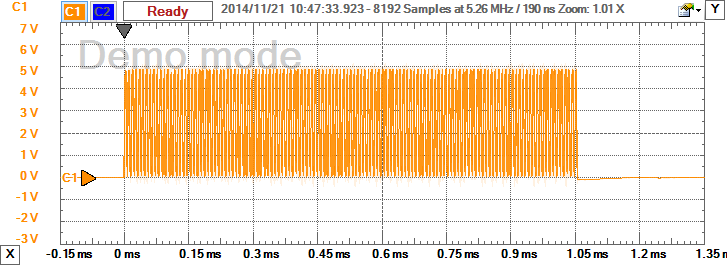
\includegraphics[width=\textwidth]{../Implementering/SW_implementering/Transmitter/sendCrossing_test}
\caption{Output på x10Data når en der skal sendes 1 i en nulgennemgang.}
\label{fig:sendCrossingtest}
\end{figure}

Frekvensen på firkantsignalet er med Analog Discovery målt til 122 kHz.

\subsubsection{waitMs()}

Hjælpemetode, som starter timer2 på 1 ms og venter til denne er færdig inden metoden forlades. 

Tiden er regnet ud ud fra følgende formel:

\begin{displaymath}
t = \frac{1}{f_{osc}} N (C - 1) = 1.00 ms
\end{displaymath}

Hvor $N$ er sat til 64 og $C$ er sat til 59. $N$ er prescaleren på clockfrekvensen for ATMega32 og $C$ er antallet af tællinger der skal til. Dvs at der skal skrives $255 - C$ til OCR2 registreret.

\subsubsection{intHandler()}

Hjælpemetode, som håndterer interrupts fra \texttt{zeroCrossDetected} benet. 

Starter med at tjekke om \texttt{start} er \texttt{TRUE}, hvis den er det fyldes \texttt{buffer} variablen med de næste nulgennemgange, som skal sendes. 

Starter med at sende MSB fra bufferen og skifte bufferen til venstre, indtil at bufferen er tom (\texttt{buffCount == 0}. Afhængigt af hvor mange mønstre (\texttt{pattCount}), som er sendt fylder den det næste mønster i bufferen. Når alle mønstre er sendt sætter den \texttt{start} til \texttt{false}.

\begin{lstlisting}
void Tx10::intHandler(){
	if (start){ //check if the Tx is supposed to transmit
		if (buffCount == 0){
			if (pattCount == 0){
				buffer = 0b11101111;
				buffCount = 4;
			}
			else if (pattCount == 1){
				buffer = house;
				buffCount = 8;
			}
			else if (pattCount == 2){
				buffer = unit;
				buffCount = 8;
			}
			else if (pattCount == 3){
				buffer = command;
				buffCount = 8;
			}
			else if (pattCount == 4){
				buffer = 0b00000011;
				buffCount = 6;
			}
			else if (pattCount == 5){
				buffer = house;
				buffCount = 8;
			}
			else if (pattCount == 6){
				buffer = unit;
				buffCount = 8;
			}
			else if (pattCount == 7){
				buffer = command;
				buffCount = 8;
			}
			else if (pattCount == 8){
				buffer = 0b11110000;
				buffCount = 4;
			}
			else if (pattCount == 9){
				start = false;
				pattCount = 0;
			}
			pattCount++;
		}
		
		if (buffCount > 0){
			sendCrossing((buffer & 0b10000000)); //Send out the MSB
			buffCount--;
			buffer = (buffer << 1); //shifts the buffer one time to the left
		}
	}
	PORTC = ~getMyTx10()->buffer; //For debugging
}
\end{lstlisting}

\subsubsection{turnAllOff()}
Metode der fylder \texttt{house} variablen med 0 (koden for at slukke alt) og sætter \texttt{start} til \texttt{TRUE}. Dette medfører at ved de eftefølgende nulgennemgange sender mønstret for at slukke alt på nettet.

\subsection{TxUART klassen (Kristian T.)} \label{TxUART}

Denne klasse er overordnet implementeret til brug i projektet ved overførsel af scenarier, men bruges også til dels til debugging af de øvrige klasser.

\subsubsection{Constructor}

Constructoren sørger for at initiere \texttt{mode} til \texttt{'i'} (idle) og initierer ellers UART på almindelig vis i henhold til protokollen.

\subsubsection{rxInt()}

Hjælpemetode, som håndterer interrupts når der modtages en \texttt{char} på UARTen. Metoden er implementeret ved at den kontrollerer hvilken tilstand, klassen er i. Hvis den er i idle udføres den kommando, som er sendt via UART. Hvis den er i receiving mode og der ikke er send 80 chars endnu, sendes der data til \texttt{Transmitter} klassen.

\begin{lstlisting}
void TxUART::rxInt(){
	char input = UDR;
	if (mode == 'i'){
		if (input == 'L'){
			bool temp = myTrans->getLockStatus();
			if (temp)
				sendChar('U');
			else
    			sendChar('L');
		}
		else if (input == 'N'){
			mode = 'r'; //put in receiving mode
			myTrans->newScen();
		}
		else if (input == 'S'){
			myTrans->stopAll();
		}
	}
	else if (mode == 'r'){
		if (charNo <= 80){
			myTrans->scenData(input);
			charNo++;
		}
		if (charNo == 80){ //end of data
			charNo = 0; //reset counter
			mode = 'i'; //put in idle mode
		}
	}
}
\end{lstlisting}

\subsubsection{sendChar(char)}

Hjælpemetode, sender en char via UART.

\subsubsection{sendString(const char * sendMe)}
Hjælpemetode til debugging, sender en række chars via UART, modtager "string literal", som de forekommer i C++. Dvs man fx kan skrive \texttt{sendString("Hello world.")}.

\subsubsection{sendNumber(int sendMe)}
Sender en integer via UART, som oversættes til ASCII-værdier først. Bruges primært til debugging af systemet.
\begin{lstlisting}
void TxUART::sendNumber(int sendMe){
	sendChar(((sendMe / 1000)%10)+48);
	sendChar(((sendMe / 100)%10)+48);
	sendChar(((sendMe / 10)%10)+48);
	sendChar(((sendMe)%10)+48);
}
\end{lstlisting}